\documentclass[11pt, notitlepage, leqno]{article}

%package imports
\usepackage[T1]{fontenc}
\usepackage[letterpaper, margin=1in]{geometry}  %for letter-sized paper
\usepackage{setspace}              %double spacing
\usepackage{fancyhdr}              %header capability
\usepackage{graphicx}
\usepackage{booktabs}
\usepackage{amsmath}
\usepackage{amssymb}
\usepackage{amsthm}
\usepackage{wrapfig}
\usepackage{tikz}
\usetikzlibrary{automata,positioning,arrows}
\usepackage{textcomp}

%page layout setup
\setlength{\headheight}{14.5pt}
\setlength{\headsep}{25pt}

%header setup
\pagestyle{fancyplain}
\fancyhf{}

\lhead{\fancyplain{}{\today}}                 %top left
\chead{\fancyplain{}{CPSC 121: Assignment 5}}                                 %top center
\rhead{\fancyplain{}{Calvin Cheng \& Brian Wu}}	                    %top right
\lfoot{\fancyplain{}{}}                                 %bottom left
\cfoot{\fancyplain{}{---\thepage---}}                   %bottom center
\rfoot{\fancyplain{}{}}                                 %bottom right

\renewcommand{\headrulewidth}{0pt}
\renewcommand{\footrulewidth}{0pt}

\renewcommand{\qedsymbol}{$\blacksquare$}

\newcommand{\unit}[1]{\;\textrm{#1}}
\renewcommand{\neg}{\mathord{\sim}}

\newcommand*\adjustwrapfigitem{\null\vskip-\baselineskip}

%document beginning
\begin{document}

%line spacing
\setstretch{1.0}

\begin{enumerate}

\item We conjecture that the sum follows the formula $S(n)=\frac{n}{n+1}$. Writing the given series in summation notation, we have the following equation:
\begin{align*}
	S(n) &= \sum\limits_{i=1}^n \frac{1}{i (i+1)} = \frac{n}{n+1}
\end{align*}
\begin{proof}
When $n=1$, the LHS of $S(1)$ is $\frac{1}{1 (1+1)} = \frac{1}{2}$, and the RHS is $\frac{1}{2}$, so S(1) is true.

Without loss of generality, suppose that $k$ is an arbitrary integer with $k \geq 1$ such that
\begin{align*}
S(k) = \sum\limits_{i=1}^k \frac{1}{i (i+1)} = \frac{k}{k+1}
\end{align*}
Assuming that this is true for $S(k)$, we must show that $S(k+1)$ is true:
\begin{align*}
\sum\limits_{i=1}^{k+1} \frac{1}{(i+1) (i+2)} &=  \sum\limits_{i=1}^k \frac{1}{i (i+1)} + \frac{1}{(k+1)(k+2)}\\
&= \frac{k}{k+1} + \frac{1}{(k+1)(k+2)}\\
&= \frac{k(k+2)}{(k+1)(k+2)} + \frac{1}{(k+1)(k+2)}\\
&= \frac{k^2 + 2k + 1}{(k+1)(k+2)}\\
&= \frac{(k+1)^2}{(k+1)(k+2)}\\
&= \frac{k+1}{k+2}\\
&= \frac{k+1}{(k+1)+1}\qedhere
\end{align*}
\end{proof}

\item \begin{proof}
We proceed by strong induction on $n$.

When $n=1$, $F_{1} = 1 < 2^{1}$.

When $n=2$, $F_{2} = 1 < 2^2$.

Suppose that $k$ is an arbitrary  integer with $k \geq 2$ such that $F_k < 2^k$. Assuming that this is true for all $k$ from 1 to $k$, we must show that $F_{k+1} < 2^{k+1}$:
\begin{align*}
F_{k+1} &= F_{k} + F_{k-1} \\
F_{k} + F_{k-1} &< 2^k +2^{k-1} \\
2^k +2^{k-1} &= 2^k + \frac{2^k}{2} \\
2^k + \frac{2^k}{2} &= \frac{3}{2} \cdot 2^k \\
\frac{3}{2} \cdot 2^k &< 2 \cdot 2^k \\
2 \cdot 2^k &= 2^{k+1} \qedhere
\end{align*}
\end{proof}

\item A DFA that takes in a string over the alphabet \{a, b, c\} and accepts exactly the strings that start and end with the same letter is shown below:
\begin{center}
\begin{tikzpicture}[>=stealth',shorten >=1pt,auto,node distance=2cm] 
	\node[state,initial] 		(s0) {s0}; 
	\node[state,accepting] 	(a1) [above right=of s0] {a1};
	\node[state]			(a2) [right=of a1] {a2};
	\node[state,accepting] 	(b1) [right=of s0] {b1}; 
	\node[state] 		(b2) [right=of b1] {b2}; 
	\node[state,accepting] 	(c1) [below right=of s0] {c1}; 
	\node[state] 		(c2) [right=of c1] {c2}; 
	\path[->]
	(s0) edge node {a} (a1)
	edge node {b} (b1)
	edge node [swap] {c} (c1)
	(a1) edge [loop above] node {a} ( )
	edge [bend left=10] node {b, c} (a2)
	(a2) edge [loop right] node {b, c} ( )
	edge [bend left=10] node {a} (a1)
	(b1) edge [loop above] node {b} ( )
	edge [bend left=10] node {a, c} (b2)
	(b2) edge [loop right] node {a, c} ( )
	edge [bend left=10] node {b} (b1)
	(c1) edge [loop above] node {c} ( )
	edge [bend left=10] node {a, b} (c2)
	(c2) edge [loop right] node {a, b} ( )
	edge [bend left=10] node {c} (c1);
\end{tikzpicture}
\end{center}


\item \begin{enumerate}

\item A*B+A(A+B+A)*B[AB]*

\item c*(ac|bc|c)*[ab]?

\end{enumerate}

\item 

\end{enumerate}

\end{document}